\chapter{Acquisition geometry and signal model}\label{ch:model}

\section{Formation and parameters}

One platform transmits and receives (channel~0); the other $\Nrx-1$ receivers fly behind it. Receiver $i$ is displaced by
$\bat_{,i}$ along track and by $\bxt_{,i}$ across track (horizontally, towards the scene) relative to the transmitter
(\cref{fig:geometry}). The along-track baselines satisfy the displaced phase centre (DPCA) condition (\cref{fig:dpca}), so that the
effective phase centres of the $\Nrx$ channels are uniformly spaced and the multichannel sampling is uniform at the full
PRF; the study is about the cross-track baselines, which are drawn at random in $[0,\bxt^{\max}]$ (with the largest equal
to $\bxt^{\max}$) or taken from fixed sets. Channel~0 is always the transmitter ($\bat=\bxt=0$). The parameters are listed
in \cref{tab:params}.

\begin{table}[htbp]
\centering
\caption{Parameters of the simulated system.}\label{tab:params}
\begin{tabular}{@{}l l@{}}
\toprule
Wavelength $\lambda$ & \SI{0.25}{m} \\
Platform altitude $H$ & \SI{720}{km} \\
Slant range of the reference point $r_0$ & \SI{766.2}{km} \\
Look angle $\theta$ & \SI{20}{\degree} \\
Platform velocity / effective velocity & \SI{7688.5}{m/s} / \SI{7408.5}{m/s} \\
Antenna length & \SI{12}{m} \\
Processed Doppler bandwidth $\Ba$ & \SI{1235}{Hz} \\
Full PRF & \SI{2000}{Hz} \\
Channel PRF $\PRFop=\PRF/\Nrx$ & \SI{1000}{Hz} to \SI{250}{Hz} ($\Nrx=2$ to $8$) \\
DPCA along-track spacing $2v/\PRF$ & \SI{7.69}{m} \\
Cross-track baselines $\bxt^{\max}$ & \SIlist{100;300;500}{m}, and fixed sets \\
\bottomrule
\end{tabular}
\end{table}

\begin{figure}[htbp]
\centering
% Bistatic geometry of one channel (adapted from the guides of the joint reconstruction)
\begin{tikzpicture}[x=1cm,y=1cm]
  % axes
  \coordinate (O) at (-3.4,0.2);
  \draw[->,ink,line width=0.8pt] (O) -- ++(0,4.6) node[left,nota]{$z$};
  \draw[->,ink,line width=0.8pt] (O) -- ++(-1.5,-0.5) node[below,nota]{$x$ (azimuth)};
  \draw[->,ink,line width=0.8pt] (O) -- ++(5.6,-2.0) node[below,nota]{$y$ (ground range)};
  % tracks
  \coordinate (T0) at (-4.2,2.95); \coordinate (T1) at (3.1,5.35);
  \coordinate (R0) at (-3.0,1.55); \coordinate (R1) at (4.6,4.05);
  \draw[cblue,dashed,line width=0.9pt] (T0) -- (T1) node[above,nota,text=cblue]{track of the Tx};
  \draw[corange,dashed,line width=0.9pt] (R0) -- (R1) node[right,nota,text=corange]{track of Rx$_i$};
  % platforms, paths and target
  \coordinate (Tx) at ($(T0)!0.36!(T1)$);
  \coordinate (Rx) at ($(R0)!0.70!(R1)$);
  \coordinate (CA) at ($(T0)!0.56!(T1)$);
  \coordinate (Tg) at (1.35,0.35);
  \coordinate (Gr) at (1.35,-1.25);
  \draw[cviolet,line width=0.9pt] (Tx) -- node[left=1pt,pos=0.55,nota,text=cviolet]{$r_{\mathrm T}(t)$} (Tg);
  \draw[caqua!80!black,line width=0.9pt] (Rx) -- node[right=1pt,pos=0.45,nota,text=caqua!70!black]{$r_{\mathrm R,i}(t)$} (Tg);
  \draw[cred,line width=0.9pt] (CA) -- node[right,pos=0.30,nota,text=cred]{$r_0$} (Tg);
  \fill[cblue] (CA) circle (1.8pt);
  \node[nota,text=cblue,anchor=south east] at ($(CA)+(-0.05,0.08)$) {$t=t_p$};
  \node[sat] at (Tx) {};
  \node[sat] at (Rx) {};
  \node[nota,anchor=north east] at ($(Tx)+(-0.08,-0.26)$) {Tx};
  \node[nota,below right=2pt] at (Rx) {Rx$_i$};
  \draw[->,ink,line width=0.8pt] (Tx) -- ++(-0.62,-0.20) node[above left=-2pt,nota]{$v$};
  \draw[->,ink,line width=0.8pt] (Rx) -- ++(-0.62,-0.20) node[above left=-2pt,nota]{$v$};
  \fill[ink] (Tg) circle (2pt);
  \node[nota,anchor=west] at ($(Tg)+(0.55,0.05)$) {scatterer $(x,y,h)$};
  \draw[cota] (Tg) -- node[right,nota]{$h$} (Gr);
  % baselines
  \coordinate (Ta) at ($(Tx)+(-0.42,1.28)$); \coordinate (Tb) at ($(Rx)+(-1.52,2.78)$);
  \draw[ink,dashed,line width=0.6pt] (Tx) -- (Ta);
  \draw[ink,dashed,line width=0.6pt] ($(Rx)+(-1.2,1.4)$) -- (Tb);
  \draw[cota] ($(Ta)+(0.05,-0.12)$) -- node[above,nota]{$\bat_{,i}$} ($(Tb)+(0.05,-0.12)$);
  \draw[cota] ($(T0)!0.93!(T1)+(0,-0.05)$) -- node[right,nota]{$\bxt_{,i}$} ($(R0)!0.80!(R1)+(0,0.05)$);
  \draw[cota,cred] (-4.25,0.05) -- node[left,nota,text=cred]{$H$} (-4.25,2.9);
\end{tikzpicture}

\caption[Bistatic geometry of one channel]{Geometry of one channel. The transmitter (Tx) and receiver $i$ (Rx$_i$) fly on
parallel tracks at the same altitude $H$, separated by $\bat_{,i}$ along track and $\bxt_{,i}$ across track. The echo of channel
$i$ travels $r_{\mathrm T}(t)+r_{\mathrm R,i}(t)$. The time of closest approach $t_p$ and the range $r_0$ fix the position of the
scatterer on the line; its height $h$ is what the topography adds. Not to scale.}
\label{fig:geometry}
\end{figure}

\begin{figure}[htbp]
\centering
% DPCA arrangement seen from above (adapted from the guide of the sub-aperture joint)
\begin{tikzpicture}[x=1cm,y=1cm]
  \draw[->,inkb,line width=0.6pt] (-6.6,2.3) -- (5.0,2.3) node[right,nota]{flight, $v$};
  \node[draw=ink,fill=cyellow,star,star points=5,star point ratio=2.3,inner sep=1.6pt] (tx) at (2.6,1.4) {};
  \node[nota,right=1.5mm of tx] {Tx};
  \foreach \i/\c in {0/ch0,1/ch1,2/ch2,3/ch3}{
     \pgfmathsetmacro{\xx}{2.6-1.9*\i}
     \fill[\c] (\xx,0.0) circle (4.2pt);
     \node[nota,below=2mm] at (\xx,0.0) {Rx$_\i$};
     \pgfmathsetmacro{\xc}{2.6-0.95*\i}
     \draw[\c,densely dotted,line width=0.6pt] (2.6,1.4) -- (\xx,0.0);
     \draw[\c,fill=white,line width=1pt] (\xc,0.7) circle (2.6pt);
  }
  \draw[cota] (2.6,-1.0) -- node[below,nota]{$\bat_{,1}=2d$} (0.7,-1.0);
  \draw[cota] (2.6,1.95) -- node[above,nota]{$d$} (1.65,1.95);
  \draw[cota] (1.65,1.95) -- node[above,nota]{$d$} (0.7,1.95);
  \draw[cota] (0.7,1.95) -- node[above,nota]{$d$} (-0.25,1.95);
  \node[nota,align=left,anchor=west] at (-6.6,0.75) {$\circ$ phase centre of the pair Tx--Rx$_i$\\ (mid-point): one every\\ $d=v/\PRF=\SI{3.84}{m}$};
  \begin{scope}[shift={(0,-2.9)}]
    \draw[->,inkb] (-6.6,0) -- (5.0,0) node[right,nota,align=left]{phase centres,\\ pulse after pulse};
    \foreach \p in {0,1,2}{
      \foreach \i/\c in {0/ch0,1/ch1,2/ch2,3/ch3}{
        \pgfmathsetmacro{\xx}{-5.8+3.8*\p+0.95*\i}
        \fill[\c] (\xx,0) circle (3pt);
      }
      \draw[cota] ({-5.8+3.8*\p},0.45) -- node[above,nota]{$D=v/\PRFop=\Nrx d$} ({-5.8+3.8*(\p+1)},0.45);
    }
  \end{scope}
\end{tikzpicture}

\caption[DPCA arrangement]{DPCA arrangement seen from above ($\Nrx=4$). Receiver $i$ trails the transmitter by
$\bat_{,i}=2id$, so the phase centre of the pair (the mid-point) trails it by $id$. At every pulse the four phase centres occupy
four equally spaced positions; between pulses the platform moves $D=\Nrx d$ and the pattern repeats. Together the channels sample
the ground every $d$, like a single channel at the full PRF.}
\label{fig:dpca}
\end{figure}

\section{Signal model}

The simulator works with point targets. In the 1-D study the targets lie on a terrain profile $h(x)$ along azimuth;
each target is placed on the iso-range surface of the reference point (same monostatic slant range $r_0$), so that
only its height changes the bistatic geometry. The reference point is at $x=0$, $h=0$. In the 2-D study (\cref{ch:joint2d}) the terrain
is a surface $h(x,y)$ and the data are range compressed. The azimuth signal of channel $i$ is
\begin{equation}
  s_i(t) = \sum_{p} a_p\, w(t-t_p)\, \exp\!\left(-\jj\frac{2\pi}{\lambda} \bigl[r_{\mathrm T,p}(t)+r_{\mathrm R,i,p}(t)\bigr]\right),
\end{equation}
with $a_p$ the complex amplitude of scatterer $p$, $w$ the antenna pattern and $r_{\mathrm T}+r_{\mathrm R,i}$ the bistatic
path (\cref{fig:geometry}).

\section{Channel transfer functions and the coefficients \texorpdfstring{$C_0$, $C_1$, $C_2$, $\Delta t$}{C0, C1, C2, Delta t}}\label{sec:coeffs}

The reconstruction (\cref{ch:recon}) needs, for every channel $i$, its transfer function $H_i(f)$: the factor by which the
Doppler spectrum of channel $i$ differs from the spectrum the monostatic system (transmitter and receiver at the
transmitter) would record for the same scatterer. This section derives $H_i$ from the range histories of the reference
point; the derivation follows the Doppler-domain approach of \cite{Sakar2020tgrs,Sakar2022thesis}.

\paragraph{Step 1: two parabolas (time domain).} Let $M(t)=2r_{\mathrm T}(t)$ be the monostatic path and
$B_i(t)=r_{\mathrm T}(t)+r_{\mathrm R,i}(t)$ the bistatic path of channel $i$, both for the reference point. Over the aperture
each is well described by a parabola around its own minimum:
\begin{equation}
  M(t)\approx M_{\min}+m_2\,(t-t_M)^2, \qquad B_i(t)\approx B_{i,\min}+b_{2,i}\,(t-t_{B,i})^2 ,
  \label{eq:parabolas}
\end{equation}
where $M_{\min}$, $B_{i,\min}$ are the smallest path lengths [m], $t_M$, $t_{B,i}$ the times at which they occur [s] and
$m_2$, $b_{2,i}$ the curvatures [m/s$^2$]. The corresponding azimuth signals are
$s_M(t)=w(t)\exp[-\jj 2\pi M(t)/\lambda]$ and $s_i(t)=w(t)\exp[-\jj 2\pi B_i(t)/\lambda]$.

\paragraph{Step 2: from time to Doppler (stationary phase).} For a signal $\exp[-\jj2\pi P(t)/\lambda]$ with a parabolic path
$P(t)=P_{\min}+p_2(t-t_P)^2$, the instantaneous frequency is
\begin{equation}
  f(t)=-\frac{1}{\lambda}\frac{\mathrm dP}{\mathrm dt}=-\frac{2p_2}{\lambda}(t-t_P)
  \quad\Longrightarrow\quad t_f=t_P-\frac{\lambda f}{2p_2},
\end{equation}
so every Doppler frequency $f$ is produced at one time $t_f$ (the same relation as the ruler \eqref{eq:ruler} of \cref{ch:recon}). By the
principle of stationary phase the phase of the spectrum at $f$ is the phase of the signal at $t_f$ minus $2\pi f t_f$. With
$P(t_f)=P_{\min}+\lambda^2f^2/(4p_2)$,
\begin{equation}
  \Psi_P(f) = -\frac{2\pi}{\lambda}P(t_f)-2\pi f t_f
  = -2\pi\Bigl[\frac{P_{\min}}{\lambda}+t_P\,f-\frac{\lambda f^2}{4p_2}\Bigr].
  \label{eq:posp}
\end{equation}
The amplitude of the spectrum is set by the antenna pattern and is the same for the two paths.

\paragraph{Step 3: the ratio of the two spectra (Doppler domain).} Applying \eqref{eq:posp} to $B_i$ and to $M$ and taking
the difference of the phases gives the transfer function of channel $i$:
\begin{equation}
  H_i(f)=\e^{\jj[\Psi_{B_i}(f)-\Psi_M(f)]}
  =\exp\!\Bigl(-\jj2\pi\Bigl[\frac{C_{0,i}}{\lambda}+(\Delta t_i-C_{1,i})\,f+C_{2,i}\,\lambda f^2\Bigr]\Bigr),
  \label{eq:Hi}
\end{equation}
with
\begin{equation}
  C_{0,i}=B_{i,\min}-M_{\min},\qquad
  \Delta t_i-C_{1,i}=t_{B,i}-t_M,\qquad
  C_{2,i}=\frac{1}{4m_2}-\frac{1}{4b_{2,i}} .
  \label{eq:coeffs}
\end{equation}
In the simulator the two paths are sampled at the full PRF: $\Delta t_i$ is the time between the samples where $M$ and $B_i$
are smallest and $C_{1,i}$ the sub-sample correction given by the linear terms of the two fitted parabolas, so that
$\Delta t_i-C_{1,i}$ is the time between the two minima.

\paragraph{Physical meaning.} Each coefficient corresponds to one effect of the bistatic geometry:
\begin{itemize}
  \item $C_{0,i}$ [m], the difference of the shortest paths, is a \emph{constant phase} $2\pi C_{0,i}/\lambda$. It is set by
        the cross-track baseline, and it is the coefficient that changes with the height of the scatterer (\cref{sec:dc0}).
  \item $\Delta t_i-C_{1,i}$ [s], the delay between the two minima, is a \emph{linear phase} in Doppler, i.e.\ a shift in time.
        It is set by the along-track baseline ($\approx\bat_{,i}/(2v)$) and is what makes the channels sample the azimuth signal at
        displaced positions (DPCA).
  \item $C_{2,i}$ [s$^2$/m], the difference of the inverse curvatures, is a \emph{quadratic phase}: a small residual azimuth chirp.
\end{itemize}
For a scatterer other than the reference point the same derivation holds with its own paths; what changes, to first order, is
$C_{0,i}$ (\cref{sec:dc0}).

\Cref{fig:coeffsref} shows the four coefficients of the reference point. $C_0$ is the difference of the closest-approach
distances of the receiver and of the transmitter, $\approx-\bxt\sin\theta$ ($\SI{-171}{m}$ for $\bxt=\SI{500}{m}$), and does
not depend on $\bat$; $\Delta t=\bat/(2v)$ (\SIlist{0.5;1.0;1.5}{ms} for the three DPCA receivers) and does not depend on $\bxt$;
$C_1$ is below \SI{0.2}{\micro s} and $C_2$ below \SI{4e-7}{s^2/m}, which at the edge of the processed band, $f=\Ba/2$, give phases
of $2\pi C_1 f<\SI{1e-3}{rad}$ and $2\pi C_2\lambda f^2\approx\SI{0.2}{rad}$. \Cref{fig:rangefit} checks the parabolic model
\eqref{eq:parabolas} for one target: the bistatic minus the monostatic path varies by a few millimetres over the aperture
(\SI{5.6}{mm} for $\bxt=\SI{300}{m}$) and the parabola reproduces it within $10^{-4}$\,\si{mm}.

\begin{figure}[htbp]
\centering
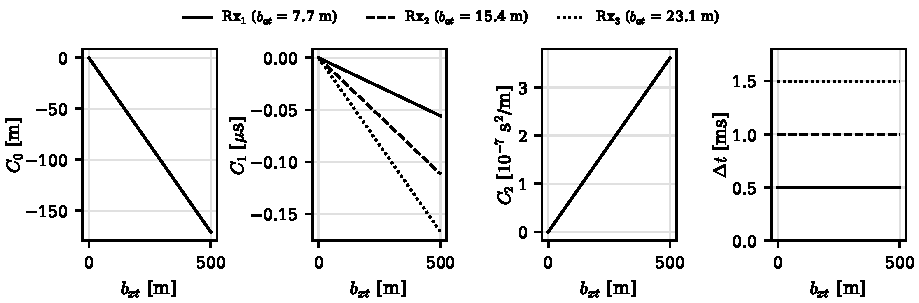
\includegraphics[width=\linewidth]{figures/coeffs_reference_point.pdf}
\caption[Coefficients of the reference point]{$C_0$, $C_1$, $C_2$ and $\Delta t$ of the reference point for the receivers
1, 2 and 3 of the DPCA formation ($\bat=\SIlist{7.7;15.4;23.1}{m}$), as a function of the cross-track baseline $\bxt$
(the same for the three receivers). The three curves of $C_0$ and of $C_2$ coincide.}
\label{fig:coeffsref}
\end{figure}

\begin{figure}[htbp]
\centering
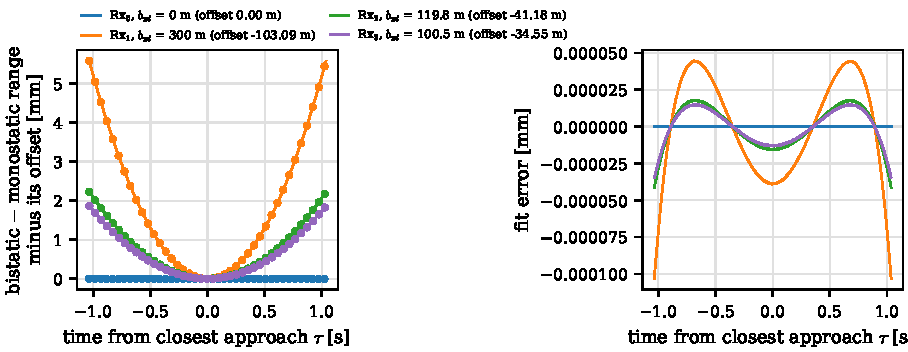
\includegraphics[width=\linewidth]{figures/range_history_fit.pdf}
\caption[Bistatic minus monostatic path and its parabola]{One target at $x=0$, $h=\SI{500}{m}$, four channels with
$\bxt=[0,300,119.8,100.5]$\,\si{m}. Left: bistatic minus monostatic path of every channel against the time from closest
approach, minus its constant offset ($C_0$, given in the legend); dots: simulated geometry; lines: the fitted parabola.
Right: difference between the simulated curve and the parabola.}
\label{fig:rangefit}
\end{figure}

\section{The topographic residual \texorpdfstring{$\dC$}{Delta C0}}\label{sec:dc0}

For a scatterer at height $h$ the coefficient $C_0$ of channel $i$ differs from the one of the reference point. The
difference is the \emph{topographic residual}
\begin{equation}
  \Delta C_{0,i}(h) = C_{0,i}(\text{scatterer}) - C_{0,i}(\text{reference point}) \approx -\frac{\bxt_{,i}\, h}{r_0 \tan\theta},
  \qquad
  \varphi_i(h) = \frac{2\pi}{\lambda}\Delta C_{0,i}(h),
  \label{eq:dc0}
\end{equation}
i.e.\ the interferometric phase of the cross-track baseline; it vanishes for the transmitter channel ($\bxt=0$),
since the targets are on the iso-range surface. The simulator computes $\Delta C_{0,i}$ exactly from the range
histories; the approximation \eqref{eq:dc0} agrees within about \SI{2}{\percent}. For a scatterer at \SI{500}{m} and $\bxt=[63.7, 27.0, 4.1, 1.7]$\,\si{m} the residuals are
$[-113.9,-48.2,-7.3,-3.0]$\,\si{mm}, i.e.\ up to half a wavelength. The other coefficients change much less with height:
the topography acts as a channel-dependent \emph{constant} phase over the aperture of each scatterer, a fact used by the
joint reconstruction (\cref{ch:joint}). \Cref{fig:coeffsres} quantifies this: up to \SI{3}{km} of height and
$\bxt=\SI{500}{m}$, $\Delta C_0$ follows \eqref{eq:dc0} within a few per cent, and at the edge of the processed band the phase
produced by $\Delta C_0$ (about \SI{80}{rad} at \SI{3}{km} with $\bxt=\SI{300}{m}$) is four orders of magnitude larger than the
one produced by $\Delta C_2$ (\SI{4e-3}{rad}) and seven larger than the one produced by $\Delta C_1$ (\SI{4e-6}{rad}); $\Delta t$
does not change with height.

\begin{figure}[htbp]
\centering
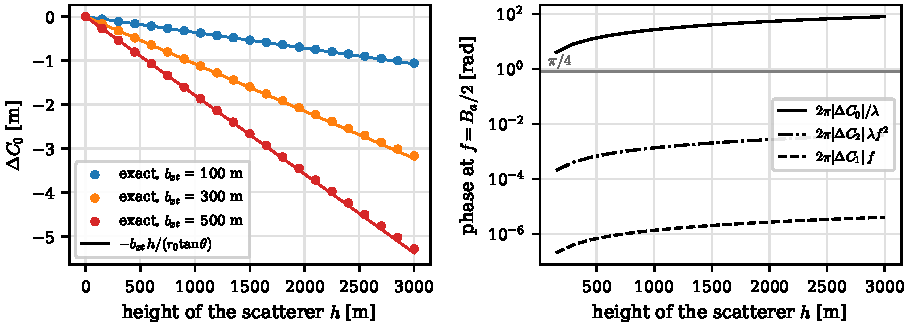
\includegraphics[width=\linewidth]{figures/coeffs_residual_height.pdf}
\caption[Change of the coefficients with the height of the scatterer]{Change of the coefficients of receiver~1 when the
scatterer is at height $h$ instead of the reference point. Left: $\Delta C_0$ (dots: exact, from the range histories; lines:
\eqref{eq:dc0}) for three cross-track baselines. Right ($\bxt=\SI{300}{m}$): phase produced by each term of \eqref{eq:Hi} at the
edge of the processed band, $f=\Ba/2$, on a logarithmic scale.}
\label{fig:coeffsres}
\end{figure}

\Cref{fig:crosstrack} shows where \eqref{eq:dc0} comes from. Moving from the reference point to a scatterer at height $h$ on
the same range arc of the transmitter is a displacement $s=h/\sin\theta$ perpendicular to the line of sight of the transmitter,
which does not change its path. The line of sight of receiver $i$ is rotated by $\Delta\theta=\bxt_{,i}\cos\theta/r_0$, so its
path changes by $s\,\Delta\theta=\bxt_{,i}h/(r_0\tan\theta)$.

\begin{figure}[htbp]
\centering
% Plane perpendicular to the track and zoom around the scatterer: origin of Delta C0 (adapted from the guides)
\begin{tikzpicture}[x=0.8cm,y=0.8cm]
  \def\rr{5.6}\def\ha{5.0}
  \coordinate (Tx) at (0,\ha);
  \coordinate (Rx) at (1.35,\ha);
  \pgfmathsetmacro{\zg}{\ha-\rr*cos(33)}
  \pgfmathsetmacro{\zp}{\ha-\rr*cos(50)}
  \pgfmathsetmacro{\xq}{\rr*sin(33)}
  \pgfmathsetmacro{\xp}{\rr*sin(50)}
  \coordinate (P0) at (\xq,\zg);
  \coordinate (P1) at (\xp,\zp);
  % terrain
  \fill[terrainfill] (1.5,\zg) -- (3.2,\zg) .. controls (3.75,\zg) and (\xp-0.5,\zp) .. (P1)
     .. controls (\xp+0.55,\zp) and (5.2,\zg) .. (5.9,\zg) -- (6.7,\zg) -- (6.7,\zg-0.18) -- (1.5,\zg-0.18) -- cycle;
  \draw[terrain,line width=0.9pt] (1.5,\zg) -- (3.2,\zg) .. controls (3.75,\zg) and (\xp-0.5,\zp) .. (P1)
     .. controls (\xp+0.55,\zp) and (5.2,\zg) .. (5.9,\zg) -- (6.7,\zg);
  \draw[inkb,dashed] (-0.6,\zg) -- (6.7,\zg) node[right,nota]{$h=0$};
  % vertical and look angle
  \draw[inkb,densely dotted] (Tx) -- (0,\zg);
  \draw[inkb] (Tx) ++(-90:1.15) arc[start angle=-90,end angle=-57,radius=1.15];
  \node[nota] at ($(Tx)+(-74:1.42)$) {$\theta$};
  % arc of equal range to the Tx
  \draw[cblue!75,line width=0.7pt,densely dashed] (Tx) ++(-63:\rr) arc[start angle=-63,end angle=-31,radius=\rr];
  \node[nota,text=cblue,anchor=south west,align=left] at ($(Tx)+(-31:\rr)+(0.08,-0.05)$) {same range\\ $r_0$ to the Tx};
  % paths
  \draw[cblue,line width=0.9pt] (Tx) -- node[below,sloped,pos=0.50,nota,text=cblue]{$r_0$} (P0);
  \draw[cblue,line width=0.9pt] (Tx) -- node[above,sloped,pos=0.62,nota,text=cblue]{$r_0$} (P1);
  \draw[corange,line width=0.9pt] (Rx) -- (P0);
  \draw[corange,line width=0.9pt] (Rx) -- (P1);
  % height and displacement on the arc
  \draw[cota] (\xp,\zg) -- node[right=-1pt,nota,text=ink]{$h$} (\xp,\zp);
  \draw[cred,line width=1.5pt,->] (P0) -- node[above left=-1.5pt,pos=0.52,nota,text=cred]{$s$} ($(P0)!0.95!(P1)$);
  \fill[ink] (P0) circle (2pt);
  \fill[ink] (P1) circle (2pt);
  \node[nota,anchor=north east,align=right] at ($(P0)+(-0.12,-0.24)$) {reference\\ point};
  \node[nota,anchor=south west] at ($(P1)+(0.45,0.0)$) {scatterer};
  % platforms and baseline
  \node[sat] at (Tx) {};
  \node[sat] at (Rx) {};
  \node[nota,anchor=east] at ($(Tx)+(-0.15,0)$) {Tx};
  \node[nota,anchor=west] at ($(Rx)+(0.15,0)$) {Rx$_i$};
  \draw[cota] ($(Tx)+(0,0.42)$) -- node[above,nota]{$\bxt_{,i}$} ($(Rx)+(0,0.42)$);
  \draw[inkb,line width=0.4pt] ($(Tx)+(0,0.14)$) -- ++(0,0.38); \draw[inkb,line width=0.4pt] ($(Rx)+(0,0.14)$) -- ++(0,0.38);
  \draw[cota] (-0.95,\zg) -- node[left,nota]{$H$} (-0.95,\ha);
  % ----------------------------------------------------------- zoom around the scatterer
  \begin{scope}[shift={(11.0,1.0)}]
    \def\tq{42}\def\dq{20}\def\sq{2.5}
    \draw[rule,rounded corners=3pt,line width=0.6pt,fill=paper] (-2.45,-2.3) rectangle (4.75,4.75);
    \node[nota,anchor=north,text=ink] at (1.15,4.62) {\textbf{zoom around the scatterer}};
    \coordinate (Q0) at (0,0);
    \coordinate (Q1) at (\tq:\sq);
    \pgfmathsetmacro{\sfq}{\sq*cos(\dq)}
    \coordinate (F) at (\tq-\dq:\sfq);
    \draw[corange,dashed,line width=0.7pt] (Q0) -- ($(Q0)+(\tq-\dq:\sfq+0.75)$);
    \draw[cblue,line width=0.9pt,->] ($(Q0)+(\tq+90:2.9)$) -- ($(Q0)+(\tq+90:0.07)$);
    \draw[cblue,line width=0.9pt,->] ($(Q1)+(\tq+90:2.2)$) -- ($(Q1)+(\tq+90:0.07)$);
    \draw[corange,line width=0.9pt,->] ($(Q0)+(\tq+90-\dq:2.9)$) -- ($(Q0)+(\tq+90-\dq:0.07)$);
    \draw[corange,line width=0.9pt,->] ($(Q1)+(\tq+90-\dq:2.2)$) -- ($(Q1)+(\tq+90-\dq:0.07)$);
    \node[nota,text=cblue,anchor=south] at ($(Q0)+(\tq+90:2.95)$) {from Tx};
    \node[nota,text=corange,anchor=south] at ($(Q0)+(\tq+90-\dq:2.95)$) {from Rx$_i$};
    \draw[ink,line width=0.6pt] (Q0) ++(\tq+90-\dq:1.9) arc[start angle=\tq+90-\dq,end angle=\tq+90,radius=1.9];
    \node[nota,text=ink] at ($(Q0)+(\tq+80:2.22)$) {$\Delta\theta$};
    \draw[ink,line width=0.6pt] (Q0) ++(\tq-\dq:1.25) arc[start angle=\tq-\dq,end angle=\tq,radius=1.25];
    \node[nota,text=ink] at ($(Q0)+(\tq-10:1.58)$) {$\Delta\theta$};
    \draw[cblue,line width=0.5pt] ($(Q0)+(\tq:0.22)$) -- ++(\tq+90:0.22) -- ++(\tq:-0.22);
    \draw[corange,line width=0.5pt] ($(F)+(\tq-\dq:-0.2)$) -- ++(\tq-\dq+90:0.2) -- ++(\tq-\dq:0.2);
    \draw[cred,line width=1.5pt,->] (Q0) -- node[above left=-1.5pt,pos=0.62,nota,text=cred]{$s$} ($(Q0)!0.96!(Q1)$);
    \draw[corange!85!black,line width=2.6pt] (Q1) -- (F);
    \node[nota,text=corange!80!black,anchor=west] at ($(Q1)!0.5!(F)+(0.12,0.05)$) {$s\,\Delta\theta$};
    \fill[ink] (Q0) circle (2pt);
    \fill[ink] (Q1) circle (2pt);
    \node[nota,anchor=north,align=center] at ($(Q0)+(-0.25,-0.14)$) {reference\\ point};
    \node[nota,anchor=south west] at ($(Q1)+(0.12,0.05)$) {scatterer};
    \node[nota,anchor=north,text=ink,align=center] at (1.15,-1.12) {$\Delta\theta=\dfrac{\bxt_{,i}\cos\theta}{r_0}$,\qquad
       $s=\dfrac{h}{\sin\theta}$};
  \end{scope}
\end{tikzpicture}

\caption[Origin of the topographic residual]{Left: plane perpendicular to the track (not to scale). The reference point and
the scatterer are at the same range $r_0$ from the transmitter, at different heights: climbing $h$ along the arc is a displacement
$s=h/\sin\theta$. Right: zoom around the scatterer. Since $s\ll r_0$ the lines of sight of each platform to the two points are
parallel; $s$ is perpendicular to the line of sight of the transmitter, but the one of the receiver is rotated by $\Delta\theta$,
and its path becomes $s\,\Delta\theta$ shorter (thick orange segment).}
\label{fig:crosstrack}
\end{figure}

\begin{figure}[htbp]
\centering
\begin{tikzpicture}
\begin{axis}[
  width=0.55\linewidth, height=5.6cm,
  xlabel={height above the reference $h$ [m]}, ylabel={$|\varphi_i|$ [deg]},
  xmin=0, xmax=1000, ymin=0, ymax=900, grid=major, grid style={gray!25},
  legend pos=outer north east, legend style={font=\small,draw=none},
  domain=0:1000, samples=2]
  \addplot[cnone,thick] {360*500*x/(0.25*766200*tan(20))};
  \addplot[cwhole,thick] {360*300*x/(0.25*766200*tan(20))};
  \addplot[cocc,thick] {360*100*x/(0.25*766200*tan(20))};
  \addplot[gray,dashed] {360};
  \legend{$\bxt=\SI{500}{m}$, $\bxt=\SI{300}{m}$, $\bxt=\SI{100}{m}$, one cycle}
\end{axis}
\end{tikzpicture}
\caption[Phase of the topographic residual]{Phase of the topographic residual \eqref{eq:dc0} against height. With
$\bxt=\SI{300}{m}$ the sensitivity is \SI{1.55}{\degree} per metre of height: a \SI{230}{m} hill already produces a full
cycle.}
\label{fig:dc0}
\end{figure}

The sensitivity is $\partial\varphi_i/\partial h = 2\pi\bxt_{,i}/(\lambda r_0\tan\theta)\approx\num{9.0e-5}\,\bxt_{,i}$
rad/m, which also sets the tolerance to DEM errors (\cref{sec:limits}).
